% -----------------------------------------------------------------
% Document class: Article
\documentclass[ a4paper, twoside, 11pt]{article}
\usepackage{../../macros-general}
\usepackage{../../macros-article}
\graphicspath{{./figures/}}
% Number of the handout, quiz, exam, etc.
\newcommand{\numero}{03}
\setcounter{numero}{\numero}

% -----------------------------------------------------------------
\begin{document}
\allowdisplaybreaks

% Indices
\newcommand{\iava}{$i$\tsup{ava} }
\newcommand{\iavo}{$i$\tsup{avo} }
\newcommand{\java}{$j$\tsup{ava} }
\newcommand{\javo}{$j$\tsup{avo} }
\newcommand{\kava}{$k$\tsup{ava} }
\newcommand{\kavo}{$k$\tsup{avo} }
\newcommand{\tava}{$t$\tsup{ava} }
\newcommand{\tavo}{$t$\tsup{avo} }
\newcommand{\tmava}{$(t-1)$\tsup{ava} }
\newcommand{\tmavo}{$(t-1)$\tsup{avo} }
\newcommand{\tMava}{$(t+1)$\tsup{ava} }
\newcommand{\tMavo}{$(t+1)$\tsup{avo} }

\begin{center}
\Large Modelos Estoc\'asticos (INDG-1008): Examen \numero \\[1ex]
\small \textbf{Semestre:} 2018-2019 T\'ermino I \qquad
\textbf{Instructor:} Luis I. Reyes Castro
\end{center}
\fullskip

% -----------------------------------------------------------------
\begin{problem}
Considere el tr\'amite mostrado en el siguiente diagrama de flujo: 
\begin{figure}[H]
\centering
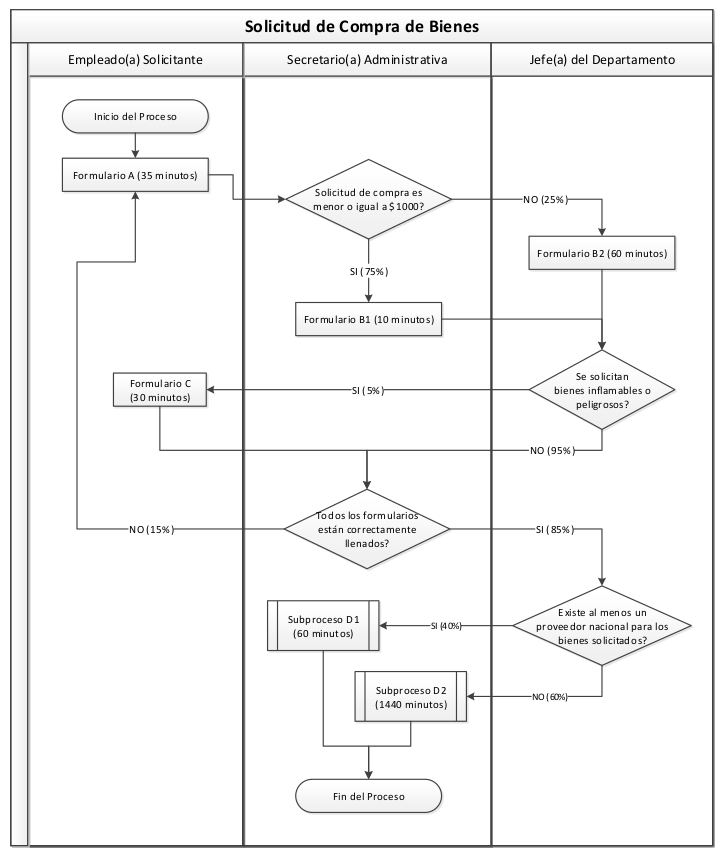
\includegraphics[width = 0.96\columnwidth]{figures/fig_burocracia.jpg}
\end{figure}
\fullcut

Con esto en mente, complete las siguientes actividades: 
\begin{enumerate}[label=\textbf{\alph*)}]
\item \textbf{[3 Puntos]} Modele el tr\'amite como una Cadena de Markov en Tiempo Discreto. 
\item \textbf{[12 Puntos]} Escriba, para cada estado, una ecuaci\'on cuya soluci\'on sea el tiempo esperado hasta el fin del proceso. 
\end{enumerate}
\QED

\end{problem}
\fullskip

% -----------------------------------------------------------------
\begin{problem}
Un psiquiatra ha pasado a\~nos estudiando pacientes que sufren de Bipolaridad Tipo II. Gracias a esta experiencia, el m\'edico ha desarrollado un modelo de Cadena de Markov de un paciente en particular. El modelo cuenta con tres estados: \'animo normal, depresi\'on, e hipoman\'ia. El modelo se comporta de la siguiente manera: 
\begin{itemize}
\item Si el paciente amanece con \'animo normal, entonces, al d\'ia siguiente: 
\begin{itemize}
\item Amanecer\'a con \'animo normal con probabilidad del 85\%. 
\item Amanecer\'a deprimido con probabilidad del 9\%. 
\item Amanecer\'a hipoman\'iaco con probabilidad del 6\%. 
\end{itemize}
\item Si el paciente amanece deprimido, entonces, al d\'ia siguiente: 
\begin{itemize}
\item Amanecer\'a deprimido con probabilidad del 67\%. 
\item Amanecer\'a con \'animo normal con probabilidad del 33\%. 
\end{itemize}
\item Si el paciente amanece hipoman\'iaco, entonces, al d\'ia siguiente: 
\begin{itemize}
\item Amanecer\'a hipoman\'iaco con probabilidad del 35\%. 
\item Amanecer\'a con \'animo normal con probabilidad del 65\%. 
\end{itemize}
\end{itemize}

Con todo esto en mente: 
\begin{enumerate}[label=\textbf{\alph*)}]
\item \textbf{[4.5 Puntos]} Escriba las ecuaciones de balance de la cadena. 
\item \textbf{[4.5 Puntos]} Encuentre la fracci\'on del tiempo (\ie de los d\'ias) que el paciente amanece en cada uno de los tres estados. 
\item \textbf{[5 Puntos]} Suponga que hoy el paciente amanece deprimido. Calcule el n\'umero esperado de d\'ias que transcurrir\'an hasta que el paciente amanezca hipoman\'iaco. 
\end{enumerate}
\QED

\end{problem}
\fullskip

% -----------------------------------------------------------------
\begin{problem}
Un sistema de colas tiene cuatro servidores y una sala de espera con capacidad para cuatro clientes. Los clientes arriban de acuerdo a un proceso Poisson con tasa media de 40 por hora, y la probabilidad de que un cliente decida ingresar al sistema decae con el n\'umero de clientes en cola de acuerdo a la ley emp\'irica: 
\[
\Pr(\text{nuevo cliente entra al sistema}) = 1 - 0.15 \, (\text{n\'umero de clientes en cola})
\]
Los tiempos de servicio tienen distribuci\'on exponencial con un valor esperado de 5 minutos. 

Con todo esto en mente, complete las siguientes actividades: 
\begin{enumerate}[label=\textbf{\alph*)}]
\item \textbf{[9 Puntos]} Modele este sistema como una Cadena de Markov en Tiempo Continuo. 
\item Suponga que usted calcul\'o correctamente la distribuci\'on estacionaria de la cadena, \ie que usted ya tiene calculados los $\pi$'s. Escriba expresiones, en t\'erminos de las probabilidades estacionarias, para las siguientes cantidades: 
\begin{enumerate}[label=\textbf{\roman*)}]
\item \textbf{[2 Puntos]} El n\'umero esperado de clientes en el sistema. 
\item \textbf{[2 Puntos]} El n\'umero esperado de clientes en cola. 
\item \textbf{[2 Puntos]} La probabilidad de que un nuevo cliente que arriba tenga que esperar en cola antes de recibir servicio. 
\end{enumerate}
\end{enumerate}
\QED

\end{problem}
\fullskip

\end{document}
